% This is samplepaper.tex, a sample chapter demonstrating the
% LLNCS macro package for Springer Computer Science proceedings;
% Version 2.21 of 2022/01/12
%
\pdfoutput=1
\RequirePackage{amsmath}
\documentclass[runningheads]{llncs}
%
\usepackage[T1]{fontenc}
% T1 fonts will be used to generate the final print and online PDFs,
% so please use T1 fonts in your manuscript whenever possible.
% Other font encondings may result in incorrect characters.
%

% other packages
\usepackage{amssymb}
\usepackage{multirow}
\usepackage[table,xcdraw]{xcolor}
\usepackage{textcomp} % for \textquotesingle
\usepackage{subfig}
\usepackage{algorithmic}
\usepackage{algorithm}
\usepackage{graphicx}
\usepackage{hyperref}
\usepackage[normalem]{ulem}
\usepackage{multirow}
\usepackage{booktabs}
\usepackage{threeparttable}
\usepackage{siunitx}
\usepackage[misc]{ifsym}
% Used for displaying a sample figure. If possible, figure files should
% be included in EPS format.
%
% If you use the hyperref package, please uncomment the following two lines
% to display URLs in blue roman font according to Springer's eBook style:
%\usepackage{color}
%\renewcommand\UrlFont{\color{blue}\rmfamily}
%
\newcommand\doubleplus{+\kern-1.3ex+\kern0.8ex}
\begin{document}
%

\title{U-Net Inspired Transformer Architecture for \\Far Horizon Time Series Forecasting}

%
\titlerunning{Yformer for Far Horizon Time Series Forecasting}
% If the paper title is too long for the running head, you can set
% an abbreviated paper title here
%
% \orcidID{0000-0001-6356-8646}
% \orcidID{1111-2222-3333-4444}
% \orcidID{0000-0002-7402-4166}
% \orcidID{2222--3333-4444-5555} 
% \orcidID{0000-0001-5729-6023}

\author{Kiran Madhusudhanan\inst{1}\Letter \and
Johannes Burchert \inst{1} \and
Nghia Duong-Trung \inst{2}\and
Stefan Born \inst{2} \and
Lars Schmidt-Thieme \inst{1} 
}
\authorrunning{K. Madhusudhanan et al.}
% First names are abbreviated in the running head.
% If there are more than two authors, 'et al.' is used.
%
\institute{Institute for Computer Science, University of Hildesheim, Hildesheim, Germany \\
\email{\{madhusudhanan, burchert, schmidt-thieme\}@ismll.uni-hildesheim.de}
\and
Technische Universit\"at Berlin, Berlin, Germany \\
\email{nghia.duong-trung@tu-berlin.de, born@math.tu-berlin.de}}

\toctitle{U-Net Inspired Transformer Architecture for Far Horizon Time Series Forecasting}
\tocauthor{Kiran~Madhusudhanan, Johannes~Burchert, Nghia~Duong-Trung, Stefan~Born and Lars~Schmidt-Thieme}

\maketitle              % typeset the header of the contribution
%
\begin{abstract}
Time series data is ubiquitous in research as well as in a wide variety of industrial applications. Effectively analyzing the available historical data and providing insights into the far future allows us to make effective decisions. Recent research has witnessed the superior performance of transformer-based architectures, especially in the regime of far horizon time series forecasting. However, the current state of the art sparse Transformer architectures fail to couple down- and upsampling procedures to produce outputs in a similar resolution as the input. We propose a U-Net inspired Transformer architecture named Yformer, based on a novel Y-shaped encoder-decoder architecture that (1) uses direct connection from the downscaled encoder layer to the corresponding upsampled decoder layer in a U-Net inspired architecture, (2) Combines the downscaling/upsampling with sparse attention to capture long-range effects, and (3) stabilizes the encoder-decoder stacks with the addition of an auxiliary reconstruction loss. Extensive experiments have been conducted with relevant baselines on three benchmark datasets, demonstrating an average improvement of 19.82, 18.41 percentage MSE and 13.62, 11.85 percentage MAE in comparison to the baselines for the univariate and the multivariate settings respectively.

\keywords{Time series Forecasting  \and Transformer \and U-Net}
\end{abstract}

version https://git-lfs.github.com/spec/v1
oid sha256:ba3550923926e025734949c64d4c34d8aa84385305492240716e694533934a35
size 5021


version https://git-lfs.github.com/spec/v1
oid sha256:5638d77e93a44dc2859bfbace73d275915f2e5b8ad919b25198e4b3c3b4f853b
size 3735


version https://git-lfs.github.com/spec/v1
oid sha256:d9c64af75406281f324b5118bf0fe8f9691f9ca3f415f72e8345bc5bc50ba1a9
size 5195


version https://git-lfs.github.com/spec/v1
oid sha256:c65db184e19d9295968256baac82954360646a290daa1d6f159a97905967c0b6
size 10075


version https://git-lfs.github.com/spec/v1
oid sha256:b45aa942d6c0e3f455db0ff166e5a6f20b430799d57450ba48cf2d06763c9035
size 4908


\section{Ablation study}
\label{sec:ablation}

Additional experiments were performed on the ETTm1 datasets to analyze the different components of the Yformer model. Similar ablation experiment results for ETTh2 dataset are reported in the Appendix section for reference.

\subsection{Y-former architecture}

In this section, we attempt to understand (1) the improvement brought about by the Y-shaped model architecture, and (2) the impact of the reconstruction loss on the superiority of the Yformer model. Firstly, Figure \ref{fig:model_size_comparison} compares the model complexity for the proposed Yformer model with the Informer baseline model and demonstrates the advantage offered by the Yformer model for longer horizons. Secondly, Figures \ref{fig:ablation_archi_uni}, \ref{fig:ablation_archi_multi}, show that the Yformer architecture performs better or is comparable to the Informer throughout the entire horizon range. Moreover, for the larger horizons, the Yformer architecture without the reconstruction loss i.e. $\alpha=0$, has a clear advantage over the Informer baseline. We attribute this improvement in performance to the additional direct U-Net inspired connections within the Yformer architecture. Using feature maps at multiple resolutions offers a clear advantage by eliminating vanishing gradients and encouraging feature reuse. Figures \ref{fig:ablation_archi_uni}, \ref{fig:ablation_archi_multi} also clearly delineates the advantage offered by adding reconstruction loss as an auxiliary task for the model, by comparing Yformer with Yformer ($\alpha=0$) results. Such a multi-task approach offers regularization to the model by learning parameters that do not overfit on the future target distribution and propels the gradients towards a general distribution that can predict the history along with the future time steps.


\begin{figure}[t]
    \centering
    \begin{tabular}{c}
    
    \subfloat[ETTm1 Univariate\label{fig:ablation_archi_uni}]{%
      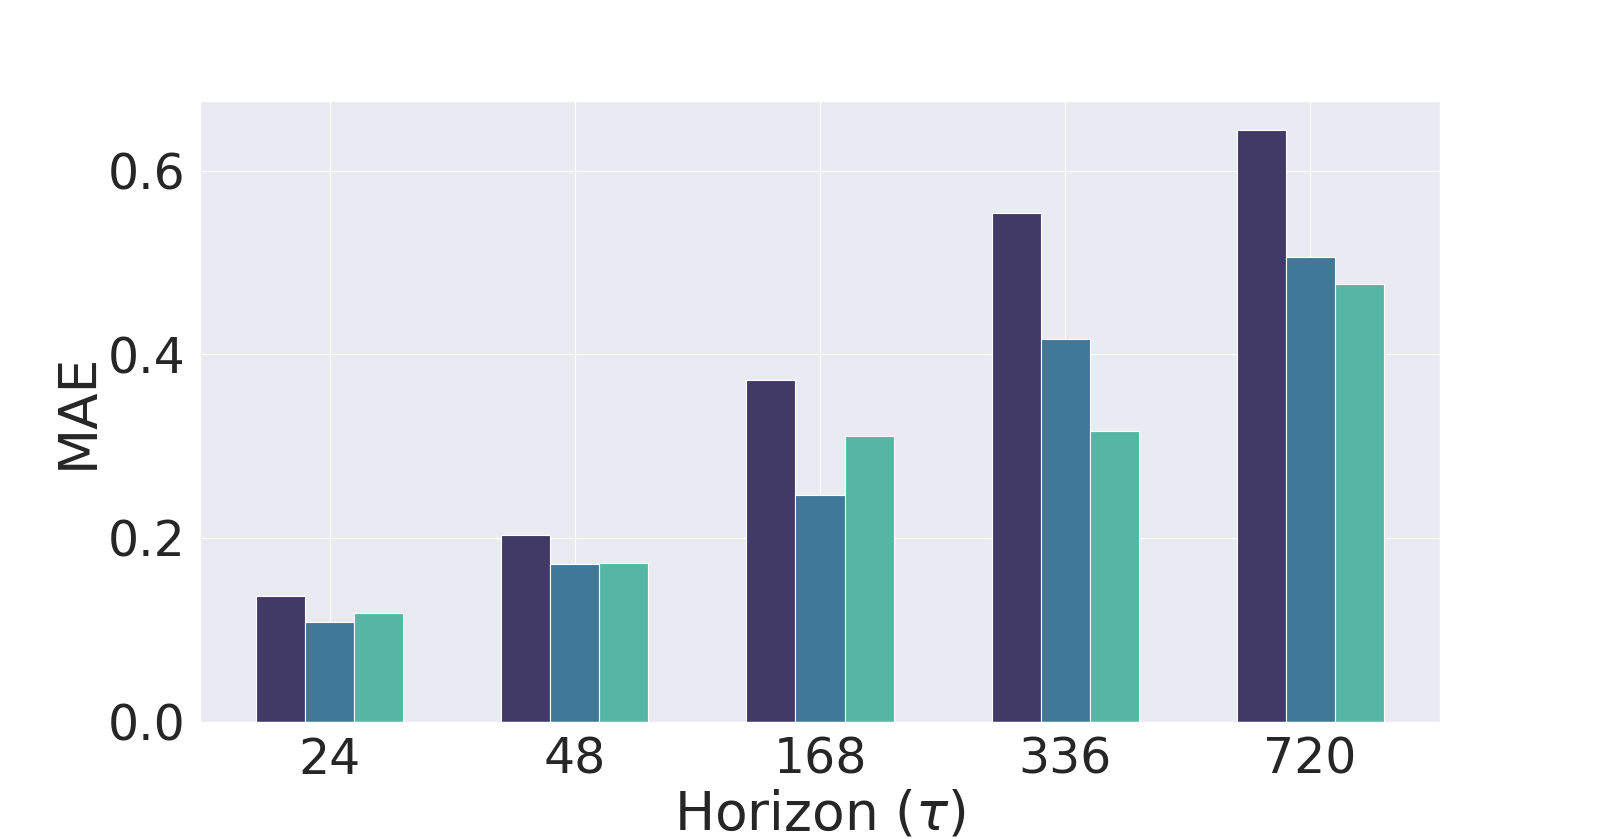
\includegraphics[width=0.40\textwidth]{figs/archi_ablation_uni_ETTm1.png}
    }

    \subfloat[ETTm1 Multivariate\label{fig:ablation_archi_multi}]{%
      \includegraphics[width=0.40\textwidth]{figs/archi_ablation_multi_ETTm1.png}
    }
    
    
    \\
    \subfloat[ETTm1 Univariate\label{fig:skipless_ablation_uni}]{%
      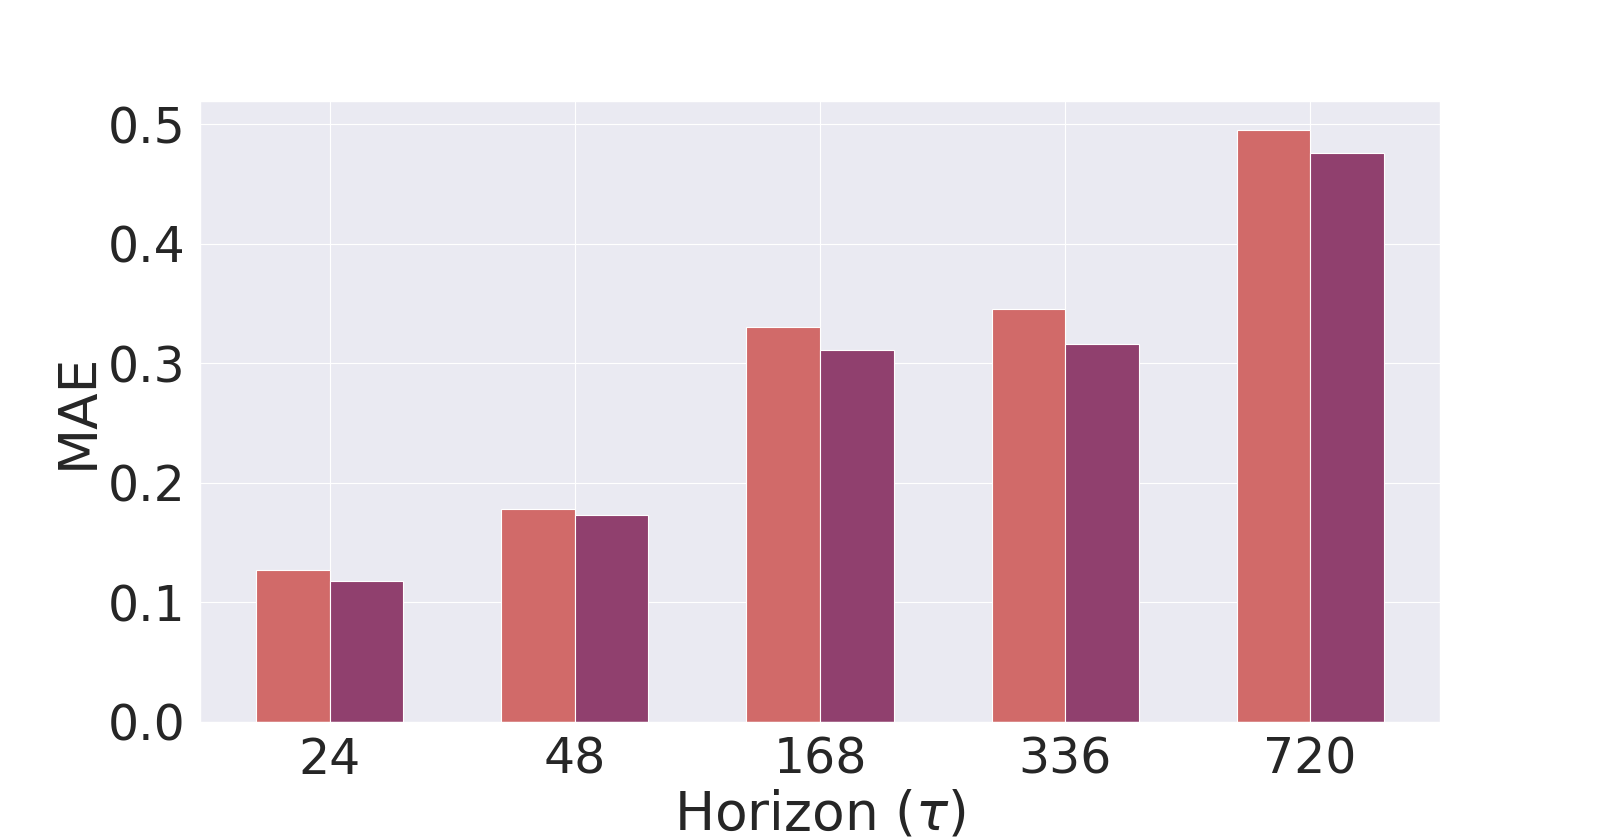
\includegraphics[width=0.40\textwidth]{figs/skipless_ablation_uni_updated.png}
    }
    \subfloat[ETTm1 Multivariate\label{fig:skipless_ablation_multi}]{%
      \includegraphics[width=0.40\textwidth]{figs/skipless_ablation_multi_updated.png}
    }
    \end{tabular}
\caption{(top) Figures \ref{fig:ablation_archi_uni}, \ref{fig:ablation_archi_multi} illustrates the reduction in MAE loss (y-axis) by  the Yformer architecture in comparison with the Informer baseline for the univariate and multivariate settings respectively. The Yformer ($\alpha=0$) represent the Yformer architecture without the reconstruction loss. (bottom) Figures \ref{fig:skipless_ablation_uni}, \ref{fig:skipless_ablation_multi} demonstrate the reduction in MAE loss (y-axis) brought by the addition of U-Net based skip connections (Yformer) to the Yformer architecture without the skip connections (Yformer$^*$). }
\label{fig:ablation_archi}
\end{figure}

\subsection{Effectiveness of the U-Net based skip connections}

To analyze the impact of U-Net based skip-connections, we conduct an ablation study on the Y-former architecture by removing the U-Net skip connections from the encoder to the decoder. We denote this model as Yformer$^*$. Figures \ref{fig:skipless_ablation_uni}, \ref{fig:skipless_ablation_multi} provides a summary of the results obtained after hyperparameter tuning the Yformer$^*$ and comparing it with the proposed Yformer model. The skip connections from the encoder to the decoder improve the performance throughout the entire horizon range for the multivariate setting and offers partial improvement for the univariate setting. Within the multivariate setting, the skip connections have a considerable impact on larger horizons and a smaller impact on the shorter horizons. This observation can be reasoned by considering the fact that long-range forecasting can utilize the additional multi-resolution encoder feature maps encoded by the U-Net based skip connections. Similar reason can be applied to the fact that U-Net based skip connections improve the performance of the multivariate setting more than that of the univariate settings.

\subsection{Reconstruction Factor}
\begin{figure}[t]
    \centering
    \begin{tabular}{c}
    \subfloat[best $\alpha$'s for Univariate\label{fig:alpha_ablation_uni}]{%
      \includegraphics[width=0.33\textwidth]{figs/factor_ablation_uni.png}
    }
    \subfloat[best $\alpha$'s for Multivariate\label{fig:alpha_ablation_multi}]{%
      \includegraphics[width=0.33\textwidth]{figs/factor_ablation_multi.png}
    }
    \subfloat[Model complexity\label{fig:model_size_comparison}]{%
      \includegraphics[width=0.34\textwidth]{figs/model_size_comparison.png}
    }
    \end{tabular}
\caption{Figures \ref{fig:alpha_ablation_uni} and \ref{fig:alpha_ablation_multi} illustrates the distribution of selected Reconstruction factor (y-axis) across the multiple horizons (x-axis). Figure \ref{fig:model_size_comparison}, compares the model size complexity (y-axis) for the multivariate setting across the multiple horizons (x-axis) for the Informer and the Yformer model.}
\label{fig:alpha_ablation}
\end{figure}


How impactful is the reconstruction factor $\alpha$ from the proposed loss in Eq. \ref{eqn:reconstruction}? We aggregated the optimal value chosen by hyperparameter tuning $\alpha$ across different datasets and summarized the distribution in Figures \ref{fig:alpha_ablation_uni} and \ref{fig:alpha_ablation_multi}. 
Interestingly, $\alpha$ value of $0.7$ is the predominant optimal setting across most horizons. Consequently, this shows that a high weight for the reconstruction loss helps the Yformer to achieve a lower loss for the future targets. Moreover, we can observe a trend that $\alpha$ is on average larger for short forecasting horizons signifying the importance of auxiliary loss for the shorter horizons. One possible reason could be that the reconstruction loss generalizes the output distribution better and avoids overfitting on short-horizon lengths. For the longer horizon forecasts, optimal $\alpha$ values are distributed on the lower and upper range of $\alpha$'s evenly, indicating that for long horizons, the reconstruction loss from long history helps for some datasets and does not for other datasets. This could be a characteristic of the dataset having a domain shift within the forecast horizon.



\section{Conclusion}

Time series forecasting is an important business and research problem that has a broad impact in today's world. This paper proposes a novel Y-shaped architecture, specifically designed for the far horizon time series forecasting problem. The study shows the importance of direct connections from the multi-resolution encoder to the decoder and reconstruction loss for the task of time series forecasting. The Yformer couples the U-Net architecture from the image segmentation domain on a sparse transformer model and empirically demonstrates superior performance across multiple datasets for both univariate and multivariate settings. We believe that our work provides a base for future research in the direction of using efficient U-Net based skip connections and the use of reconstruction loss as an auxiliary loss within the time series forecasting community.

\subsubsection{Acknowledgements}: This work was supported by the Federal Ministry for Economic Affairs and Climate Action (BMWK), Germany, within the framework of the IIP-Ecosphere project (project number: 01MK20006D)


% % ---- Bibliography ----

% % BibTeX users should specify bibliography style 'splncs04'.
% % References will then be sorted and formatted in the correct style.

\bibliographystyle{splncs04}
\begin{thebibliography}{10}
    \providecommand{\url}[1]{\texttt{#1}}
    \providecommand{\urlprefix}{URL }
    \providecommand{\doi}[1]{https://doi.org/#1}
    
    \bibitem{layernorm}
    Ba, L.J., Kiros, J.R., Hinton, G.E.: Layer normalization. CoRR  (2016)
    
    \bibitem{BoxArima}
    Box, G.E.P., Jenkins, G.M.: Some recent advances in forecasting and control.
      Journal of the Royal Statistical Society. Series C (Applied Statistics)
      (1968)
    
    \bibitem{camacho2013model}
    Camacho, E.F., Alba, C.B.: Model predictive control. Springer science \&
      business media (2013)
    
    \bibitem{cao2018brits}
    Cao, W., Wang, D., Li, J., Zhou, H., Li, L., Li, Y.: Brits: Bidirectional
      recurrent imputation for time series. In: NeurIPS (2018)
    
    \bibitem{cirstea2022triformer}
    Cirstea, R.G., Guo, C., Yang, B., Kieu, T., Dong, X., Pan, S.: Triformer:
      Triangular, variable-specific attentions for long sequence multivariate time
      series forecasting. IJCAI  (2022)
    
    \bibitem{elu}
    Clevert, D., Unterthiner, T., Hochreiter, S.: Fast and accurate deep network
      learning by exponential linear units (elus). In: ICLR (2016)
    
    \bibitem{10.1145/3292500.3330662}
    Fan, C., Zhang, Y., Pan, Y., Li, X., Zhang, C., Yuan, R., Wu, D., Wang, W.,
      Pei, J., Huang, H.: Multi-horizon time series forecasting with temporal
      attention learning. In: SIGKDD (2019)
    
    \bibitem{he2016deep}
    He, K., Zhang, X., Ren, S., Sun, J.: Deep residual learning for image
      recognition. In: CVPR (2016)
    
    \bibitem{huang2017densely}
    Huang, G., Liu, Z., Van Der~Maaten, L., Weinberger, K.Q.: Densely connected
      convolutional networks. In: CVPR (2017)
    
    \bibitem{hyndman2018forecasting}
    Hyndman, R.J., Athanasopoulos, G.: Forecasting: principles and practice. OTexts
      (2018)
    
    \bibitem{Jarrett2020Target-Embedding}
    Jarrett, D., van~der Schaar, M.: Target-embedding autoencoders for supervised
      representation learning. In: ICLR (2020)
    
    \bibitem{jawed2019multi}
    Jawed, S., Rashed, A., Schmidt-Thieme, L.: Multi-step forecasting via
      multi-task learning. In: IEEE Big Data (2019)
    
    \bibitem{tungbcc19}
    Kieu, T., Yang, B., Guo, C., S.~Jensen, C.: Outlier detection for time series
      with recurrent autoencoder ensembles. In: IJCAI (2019)
    
    \bibitem{kitaev2020reformer}
    Kitaev, N., Kaiser, L., Levskaya, A.: Reformer: The efficient transformer. In:
      ICLR (2020)
    
    \bibitem{alexnet}
    Krizhevsky, A., Sutskever, I., Hinton, G.E.: Imagenet classification with deep
      convolutional neural networks. NeurIPS  (2012)
    
    \bibitem{lai2018modeling}
    Lai, G., Chang, W.C., Yang, Y., Liu, H.: Modeling long-and short-term temporal
      patterns with deep neural networks. In: SIGIR (2018)
    
    \bibitem{le2018supervised}
    Le, L., Patterson, A., White, M.: Supervised autoencoders: Improving
      generalization performance with unsupervised regularizers. NeurIPS  (2018)
    
    \bibitem{li2019enhancing}
    Li, S., Jin, X., Xuan, Y., Zhou, X., Chen, W., Wang, Y.X., Yan, X.: Enhancing
      the locality and breaking the memory bottleneck of transformer on time series
      forecasting. NeurIPS  (2019)
    
    \bibitem{tft}
    Lim, B., Arık, S.{\"O}., Loeff, N., Pfister, T.: Temporal fusion transformers
      for interpretable multi-horizon time series forecasting. Int. J. Forecast.
      (2021)
    
    \bibitem{lin2017feature}
    Lin, T.Y., Doll{\'a}r, P., Girshick, R., He, K., Hariharan, B., Belongie, S.:
      Feature pyramid networks for object detection. In: CVPR (2017)
    
    \bibitem{nbeats}
    Oreshkin, B.N., Carpov, D., Chapados, N., Bengio, Y.: N-beats: Neural basis
      expansion analysis for interpretable time series forecasting. In: ICLR (2020)
    
    \bibitem{perslev2019u}
    Perslev, M., Jensen, M., Darkner, S., Jennum, P.J., Igel, C.: U-time: A fully
      convolutional network for time series segmentation applied to sleep staging.
      NeurIPS  (2019)
    
    \bibitem{petit2021u}
    Petit, O., Thome, N., Rambour, C., Themyr, L., Collins, T., Soler, L.: U-net
      transformer: Self and cross attention for medical image segmentation. In:
      International Workshop on MLMI (2021)
    
    \bibitem{qin2017dual}
    Qin, Y., Song, D., Chen, H., Cheng, W., Jiang, G., Cottrell, G.W.: A dual-stage
      attention-based recurrent neural network for time series prediction. In:
      IJCAI (2017)
    
    \bibitem{RangapuramDeepState}
    Rangapuram, S.S., Seeger, M.W., Gasthaus, J., Stella, L., Wang, Y.,
      Januschowski, T.: Deep state space models for time series forecasting. In:
      NeurIPS (2018)
    
    \bibitem{ronneberger2015u}
    Ronneberger, O., Fischer, P., Brox, T.: U-net: Convolutional networks for
      biomedical image segmentation. In: MICCAI (2015)
    
    \bibitem{sagheer2019time}
    Sagheer, A., Kotb, M.: Time series forecasting of petroleum production using
      deep lstm recurrent networks. Neurocomputing  (2019)
    
    \bibitem{salinas2020deepar}
    Salinas, D., Flunkert, V., Gasthaus, J., Januschowski, T.: Deepar:
      Probabilistic forecasting with autoregressive recurrent networks. Int. J.
      Forecast.  (2020)
    
    \bibitem{sezer2020financial}
    Sezer, O.B., Gudelek, M.U., Ozbayoglu, A.M.: Financial time series forecasting
      with deep learning: A systematic literature review: 2005--2019. Applied soft
      computing  (2020)
    
    \bibitem{vaswani2017attention}
    Vaswani, A., Shazeer, N., Parmar, N., Uszkoreit, J., Jones, L., Gomez, A.N.,
      Kaiser, {\L}., Polosukhin, I.: Attention is all you need. In: NeurIPS (2017)
    
    \bibitem{wang2020linformer}
    Wang, S., Li, B.Z., Khabsa, M., Fang, H., Ma, H.: Linformer: Self-attention
      with linear complexity. ArXiv  (2020)
    
    \bibitem{wang2019srn}
    Wang, Y., Tao, X., Shen, X., Jia, J.: Wide-context semantic image
      extrapolation. In: CVPR (2019)
    
    \bibitem{wang2017time}
    Wang, Z., Yan, W., Oates, T.: Time series classification from scratch with deep
      neural networks: A strong baseline. In: IJCNN (2017)
    
    \bibitem{wu2021autoformer}
    Wu, H., Xu, J., Wang, J., Long, M.: Autoformer: Decomposition transformers with
      auto-correlation for long-term series forecasting. NeurIPS  (2021)
    
    \bibitem{zhou2020informer}
    Zhou, H., Zhang, S., Peng, J., Zhang, S., Li, J., Xiong, H., Zhang, W.:
      Informer: Beyond efficient transformer for long sequence time-series
      forecasting. In: AAAI (2021)
    
    \bibitem{zhou2021nnformer}
    Zhou, H.Y., Guo, J., Zhang, Y., Yu, L., Wang, L., Yu, Y.: nnformer: Interleaved
      transformer for volumetric segmentation. ArXiv  (2021)
    
    \bibitem{ZOU201939}
    Zou, X., Wang, Z., Li, Q., Sheng, W.: Integration of residual network and
      convolutional neural network along with various activation functions and
      global pooling for time series classification. Neurocomputing  (2019)
    
    \end{thebibliography}
    


\clearpage
version https://git-lfs.github.com/spec/v1
oid sha256:acf082414844baa070da9f4ef2b0d8ae3ee7cf1d71ef93bfb27903fab9bf8ac2
size 6711


    

\end{document}
